\chapter{分析与改进}

\subsection{CTPN}
\noindent

\begin{figure}[hp]
    \centering
    
\includegraphics[scale=0.5]{rpn.eps}
    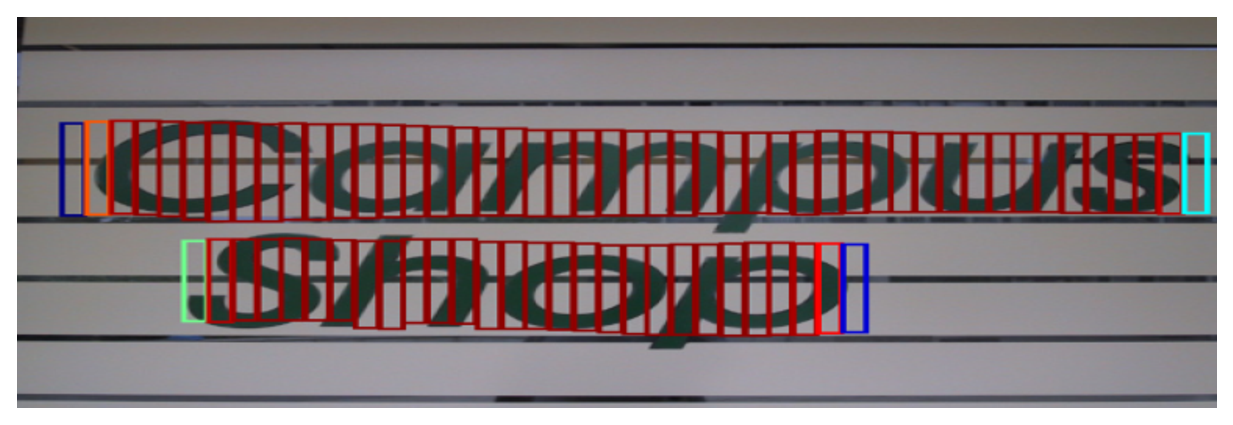
\includegraphics[scale=0.5]{ctpn.eps}
    \caption{CTPN proposals}
    \label{fig:label}
\end{figure}

在独立做完以上工作后,查阅论文时发现在OCR领域已有许多类似的工作。传统的做法即是先做单词分割,再使用分类器进行分割。如CTPN\cite{ctpn}、CRNN等。CRNN主要做的是文字识别工作,而CTPN做的是文字检测。

CTPN做的是自然场景图象中的水平文字检测,主要是在Faster RCNN的基础上结合LSTM生成的模型。首先是通过VGG提取特征,将生成的feature map经过一些处理后输入双向LSTM中,生成既包含CNN学习到的空间特征,也包含LSTM学习到的序列特征的特征图。再将特征图通过类似Faster RCNN的RPN网络,获得text proposals。CTPN生成的是宽度不变的anchor,通过寻找anchor中心和高度来获得一个小尺寸的text proposal,如图2,上面是传统的RPN的输出,下面为CTPN输出的text proposals,可以看见一个文本有许多小宽度的proposals,接下来只需要通过文本线构造办法,将这些连接起来形成一个文本检测框。

CTPN的工作是自然场景图象中的文字检测,用在我们的论文图片中有大材小用的样子。但是CTPN的方法给予了我一些启发。在处理单词图片时我们直接将单词图片resize到了固定长宽,如果我们不是resize,而是以一定宽度做crop,甚至以字母图片为基础来进行训练,同时在网络中引入RNN来获得序列信息,对效果也许会有提升。
